\documentclass[notes.tex]{subfiles}

\begin{document}

\chapter{Monoidal categories}\label{sec:monoidalcategories}

\section{Structure}

\subsection{Basic definitions}\label{ssc:basic_definitions}

Many types of mathematical structures can be combined to form new ones. For example: 
\begin{itemize}
  \item The tensor product allows us to use two vector spaces to produce a new one, as does the direct sum.

  \item The Cartesian product and the disjoint union of sets produce a new set out of two given ones.
\end{itemize}

In each of these cases, there is a natural isomorphisms making this combination associative, and an identity object which acts, up to natural isomorphism, as a left and right identity. This means that each of these operations gives the collection of all objects the structure of a monoid.

A monoidal category will be a category in which the objects have the structure of a monoid, i.e.\ there is a suitably defined `multiplication' (usually written $\otimes$) which is unital (with unit $1$) and associative. The prototypical example of categorical multiplication is the product (see \hyperref[eg:universalpropertyofproducts]{Example~\ref*{eg:universalpropertyofproducts}}), although it is far from the only one.

When put like this, monoidal categories don't sound like complicated entities, and indeed in practice they are not. However, there is a lot of subtlety in making associativity play well with multiplication by units. Since we are in a category, demanding that our multiplication be associative `on the nose,' i.e.\ that, for example,
\begin{equation*}
  (V \otimes 1) \otimes (W \otimes T) \qquad\text{and}\qquad (V \otimes W) \otimes T
\end{equation*}
should be literally equal, is too draconian, not to mention difficult to interpret. The natural weakening of this is to demand that these be merely isomorphic, but this is far too weak: for vector spaces, for example, this requires only that the dimension be the same. Even natural isomorphism is not quite strong enough.

The correct way of solving this problem is by demanding that certain diagrams, called \emph{coherenece diagrams}, commute. These diagrams then force other diagrams to commute in a way that solves our problem, as Mac Lane showed in the so-called \emph{Mac Lane's Coherence Theorem}.

\begin{definition}[monoidal category]
  \label{def:monoidalcategory}
  A \defn{monoidal category} is a category $\mathsf{C}$ equipped with a monoidal structure. A monoidal structure is the following:
  \begin{itemize}
    \item A bifunctor (\hyperref[def:bifunctor]{Definition~\ref*{def:bifunctor}}) $\otimes\colon \mathsf{C} \times \mathsf{C} \to \mathsf{C}$ called the \emph{tensor product},
    \item An object $I$ called the \emph{unit object}, and
    \item Three natural isomorphisms (\hyperref[def:naturalisomorphism]{Definition~\ref*{def:naturalisomorphism}}) subject to coherence conditions expressing the fact that the tensor product
      \begin{itemize}
        \item is associative: there is a natural isomorphism $\alpha$ called the \emph{associator}, with components
          \begin{equation*}
            \alpha_{A,B,C}\colon (A\otimes B)\otimes C \xrightarrow{\sim} A \otimes (B \otimes C)
          \end{equation*}

        \item has left and right identity: there are two natural isomorphisms $\lambda$ and $\rho$ respectively called the \emph{left unitor} and \emph{right unitor} with components
          \begin{equation*}
            \lambda_{A}\colon I \otimes A \xrightarrow{\sim} A
          \end{equation*}
          and
          \begin{equation*}
            \rho_{A}\colon A \otimes I \xrightarrow{\sim} A.
          \end{equation*}
      \end{itemize}
  \end{itemize}
  The coherence conditions are that the following diagrams commute for all $A$, $B$, $C$, and $D\in \Obj(C)$.
  \begin{itemize}
    \item The \emph{triangle diagram}
      \begin{equation*}
        \begin{tikzcd}[column sep=tiny, row sep=6ex]
          (A \otimes I) \otimes B \arrow[rr, "\alpha_{A,I,B}"] \arrow[rd, swap, "\rho_{A} \otimes \id_{B}"] & & A \otimes(I \otimes B) \arrow[ld, "\id_{A}\otimes \lambda_{B}"] \\
          & A \otimes B
        \end{tikzcd}
      \end{equation*}
    \item The \emph{home plate diagram}\footnote{Unfortunately, the home plate, as drawn, is actually upside down.} (usually the \emph{pentagon diagram})
      \begin{equation*}
        \begin{tikzcd}[row sep=huge]
          & (A \otimes (B \otimes C)) \otimes D
          \arrow[dr, "\alpha_{A,B\otimes C, D}"]
          \\
          ((A \otimes B) \otimes C) \otimes D
          \arrow[ur, "\alpha_{A,B,C}\otimes \id_{D}"]
          \arrow[dd, swap, "\alpha_{A\otimes B, C,D}"]
          & & A \otimes ((B \otimes C) \otimes D)
          \arrow[dd, "\id_{A}\otimes\alpha_{B,C,D}"]
          \\
          \\
          (A \otimes B) \otimes (C \otimes D)
          \arrow[rr, swap, "\alpha_{A,B,C\otimes D}"]
          & & A \otimes(B \otimes (C \otimes D))
        \end{tikzcd}
      \end{equation*}
  \end{itemize}

  More succinctly, a monoidal structure on a category $\mathsf{C}$ is a quintuple $(\otimes, 1, \alpha, \lambda, \rho)$.
\end{definition}

\begin{notation}
  The notation $(\otimes, 1, \alpha, \lambda, \rho)$ is prone to change. If the associator and unitors are not important, or understood from context, they are often left out. We will often say ``Let $(\mathsf{C}, \otimes, 1)$ be a monoidal category.''
\end{notation}

\begin{example}
  \label{eg:setisamonoidalcategory}
  The simplest (though not the prototypical) example of a monoidal category is $\mathsf{Set}$ with the Cartesian product. We have already studied this structure in some detail in \hyperref[sec:cartesianclosedcategories]{Section~\ref*{sec:cartesianclosedcategories}}. We check that it satisfies the axioms in \hyperref[def:monoidalcategory]{Definition~\ref*{def:monoidalcategory}}.

  \begin{itemize}
    \item The Cartesian product on $\mathsf{Set}$ \emph{is} a set-theoretic product, and can be naturally viewed, thanks to \hyperref[thm:productisafunctor]{Theorem~\ref*{thm:productisafunctor}}, as the bifunctor.

    \item Any set with one element $I = \left\{ * \right\}$ functions as the unit object.

    \item For all sets $A$, $B$, $C$
      \begin{itemize}
        \item The universal property of products gives us a natural isomorphism with components
          \begin{equation*}
            \alpha_{A,B,C}\colon (A \times B) \times C \to A \times (B \times C);\qquad ((a,b),c) \mapsto (a,(b,c)).
          \end{equation*}

        \item Since $\{*\}$ is terminal, we get an isomorphism $\lambda_{A}\colon \left\{ * \right\}\times A \to A$ which sends $(*,a) \mapsto a$.

        \item Similarly, we get a map $\rho_{A}\colon A \times\left\{ * \right\} \to A$ which sends $(a, *) \mapsto a$.
      \end{itemize}
  \end{itemize}

  The pentagon and triangle diagram commute vacuously since the cartesian product is associative.
\end{example}

\begin{lemma}
  The tensor product $\otimes$ of vector spaces is a bifunctor $\mathsf{Vect}_{k} \times \mathsf{Ve ct}_{k} \rightsquigarrow \mathsf{Vect}_{k}$.
\end{lemma}
\begin{proof}
  It is clear what the domain and codomain of the tensor product is, and how it behaves on objects and morphisms. The only non-trivial aspect is showing that the standard definition of the tensor product of morphisms respects composition, which is not difficult.
\end{proof}

\begin{example}
  \label{eg:vectisamonoidalcategory}
  The category $\mathsf{Vect}_{k}$ is a monoidal category with
  \begin{enumerate}
    \item The bifunctor $\otimes$ is given by the tensor product.

    \item The unit $1$ is given by the field $k$ regarded as a $1$-dimensional vector space over itself.

    \item The associator is the map which sends $(v_{1} \otimes v_{2}) \otimes v_{3}$ to $v_{1} \otimes (v_{2} \otimes v_{3})$. It is not \emph{a priori} obvious that this is well-defined, but it is also not difficult to check.

    \item The left unitor is the map which sends $(x, v) \in k \times V$
      to $xv \in V$.

    \item The right unitor is the map which sends
      \begin{equation*}
        (v, x) \mapsto xv.
      \end{equation*}
  \end{enumerate}
\end{example}

\begin{definition}[monoidal subcategory]
  \label{def:monoidalsubcategory}
  Let $(\mathsf{C}, \otimes, 1)$ be a monoidal category. A \defn{monoidal subcategory} of $\mathsf{C}$ is a subcategory (\hyperref[def:subcategory]{Definition~\ref*{def:subcategory}}) $\mathsf{S} \subseteq \mathsf{C}$ which is closed under the tensor product, and which contains $1$.
\end{definition}

\begin{example}
  Recall that $\mathsf{FinVect}_{k}$ is the category of finite dimensional vector spaces over a field $k$. We saw in \hyperref[eg:finvectfullsubcategoryofvect]{Example~\ref*{eg:finvectfullsubcategoryofvect}} that $\mathsf{FinVect}_{k}$ was a full subcategory of $\mathsf{Vect}_{k}$.

  We have just seen that $\mathsf{Vect}_{k}$ is a monoidal category with unit object $1 = k$. Since $k$ is a one-dimensional vector space over itself, $k \in \Obj(\mathsf{FinVect}_{k})$, and since the dimension of the tensor product of two finite-dimensional vector spaces is the product of their dimensions, the tensor product is closed in $\mathsf{FinVect}_{k}$. Hence $\mathsf{FinVect}_{k}$ is a monoidal subcategory of $\mathsf{Vect}_{k}$.
\end{example}

\begin{lemma}
  \label{lemma:leftandrightunitoragreewhenpossible}
  Let $\mathsf{C}$ be a category with monoidal structure $(\otimes, 1, \alpha, \lambda, \rho)$. Then the maps $\lambda_{1}$ and $\rho_{1}\colon 1 \otimes 1 \to 1$ agree.
\end{lemma}
\begin{proof}
  See~\cite{nlab-deligne-theorem}, Lemma 3.9.
\end{proof}

%\begin{lemma}
%  Let $\mathsf{C}$ be a category with monoidal structure $(\otimes, 1, \alpha, \lambda, \rho)$. Then for all $X$, $Y \in \Obj(\mathsf{C})$, the diagram
%  \begin{equation*}
%    \begin{tikzcd}[row sep=large]
%      (1 \otimes X) \otimes Y
%      \arrow[d, swap, "{\alpha_{1, X, Y}}"]
%      \arrow[dr, "\lambda_{X} \otimes \id_{Y}"]
%      &
%      \\
%      1 \otimes (X \otimes Y)
%      \arrow[r, swap, "\lambda_{X \otimes Y}"]
%      & X \otimes Y
%    \end{tikzcd}
%  \end{equation*}
%  commutes.
%\end{lemma}
%\begin{proof}
%
%\end{proof}
%
\begin{note}
  The triangle and pentagon diagram are the first in a long list of coherence diagrams designed to make categorical structures behave like their algebraic counterparts. For a monoid, multiplication is associative by fiat, and the extension of this to $n$-fold products follows by induction. In monoidal categories, associators are isomorphisms rather than equalities, and we have no a priori guarantee that different ways of composing associators give the same isomorphism.

  Mac Lane's coherence theorem shows us that this is exactly what the coherence diagrams guarantee.
\end{note}

\begin{theorem}[Mac Lane's coherence theorem]
  Any two ways of freely composing unitors and associators to go from one expression to another coincide.
\end{theorem}

The following definition was taken \emph{mutatis mutandis} from~\cite{baez-definitions-everyone-should-know}.
\begin{definition}[monoidal functor]
  \label{def:monoidalfunctor}
  Let $\mathsf{C}$ and $\mathsf{C}'$ be monoidal categories. A functor $\mathcal{F}\colon \mathsf{C} \rightsquigarrow \mathsf{C}'$ is \defn{lax monoidal} if it is equipped with
  \begin{itemize}
    \item a natural transformation $\Phi_{X, Y}\colon \mathcal{F}(X) \otimes \mathcal{F}(Y) \to \mathcal{F}(X \otimes Y)$, and

    \item a morphism $\varphi\colon \id_{C'} \to \mathcal{F}(\id_{C})$ such that

    \item the following diagrams commute for any $X$, $Y$, $Z \in \Obj(\mathsf{C})$.
      \begin{equation*}
        \begin{tikzcd}[row sep=huge, column sep=huge]
          (\mathcal{F}(X) \otimes \mathcal{F}(Y)) \otimes \mathcal{F}(Z)
          \arrow[r, "{\Phi_{X, Y} \otimes \id_{\mathcal{F}(Z)}}"]
          \arrow[d, swap, "\alpha_{\mathcal{F}(X), \mathcal{F}(Y), \mathcal{F}(Z)}"]
          & \mathcal{F}(X \otimes Y) \otimes \mathcal{F}(Z)
          \arrow[r, "{\Phi_{X \otimes Y, Z}}"]
          & \mathcal{F}((X \otimes Y) \otimes Z)
          \arrow[d, "{\mathcal{F}(\alpha_{X, Y, Z})}"]
          \\
          \mathcal{F}(X) \otimes (\mathcal{F}(Y) \otimes \mathcal{F}(Z))
          \arrow[r, swap, "{\id_{\mathcal{F}(X)} \otimes \Phi_{Y, Z}}"]
          & \mathcal{F}(X) \otimes \mathcal{F}(Y \otimes Z)
          \arrow[r, swap, "{\varphi_{X, Y \otimes Z}}"]
          & \mathcal{F}(X \otimes (Y \otimes Z))
        \end{tikzcd}
      \end{equation*}
      \begin{equation*}
        \begin{tikzcd}[row sep=huge, column sep=huge]
          1 \otimes \mathcal{F}(X)
          \arrow[r, "\lambda_{\mathcal{F}(X)}"]
          \arrow[d, swap, "\varphi \otimes \id_{\mathcal{F}(X)}"]
          & \mathcal{F}(X)
          \\
          \mathcal{F}(1) \otimes \mathcal{F}(X)
          \arrow[r, "{\Phi_{1, X}}"]
          & \mathcal{F}(1 \otimes X)
          \arrow[u, swap, "\mathcal{F}(\lambda_{X})"]
        \end{tikzcd}
      \end{equation*}
      \begin{equation*}
        \begin{tikzcd}[row sep=huge, column sep=huge]
          \mathcal{F}(X) \otimes 1
          \arrow[r, "\rho_{\mathcal{F}(X)}"]
          \arrow[d, swap, "\id_{\mathcal{F}(X)\otimes \varphi }"]
          & \mathcal{F}(X)
          \\
          \mathcal{F}(X) \otimes \mathcal{F}(1)
          \arrow[r, "\Phi_{X, 1}"]
          & \mathcal{F}(X \otimes 1)
          \arrow[u, swap, "F(\lambda_{X})"]
        \end{tikzcd}
      \end{equation*}
  \end{itemize}

  If $\Phi$ is a natural isomorphism and $\varphi$ is an isomorphism, then $\mathcal{F}$ is called a \defn{strong monoidal functor}.

  We will denote the above monoidal functor by $(\mathcal{F}, \Phi, \varphi)$.
\end{definition}

\begin{note}
  The above diagrams above are exactly those necessary to ensure that the monoidal structure is preserved. They do this by demanding that the associator and the unitors be $\mathcal{F}$-equivariant.
\end{note}

\begin{note}
  In much of the literature, a strong monoidal functor is simply called a monoidal functor.
\end{note}

%\begin{lemma}
%  The composition of lax (strong) monoidal functors is lax (strong) monoidal.
%\end{lemma}
%\begin{proof}
%
%\end{proof}

\begin{definition}[monoidal natural transformation]
  \label{def:monoidalnaturatransformation}
  Let $(F, \Phi, \varphi)$ and $(G, \Gamma, \gamma)$ be monoidal functors. A natural transformation $\eta: \mathcal{F} \Rightarrow \mathcal{G}$ is \defn{monoidal} if the following diagrams commute.
  \begin{equation*}
    \begin{tikzcd}[column sep=large]
      \mathcal{F}(X) \otimes \mathcal{F}(Y)
      \arrow[r, "\eta_{X} \otimes \eta_{Y}"]
      \arrow[d, swap, "{\Phi_{X, Y}}"]
      & \mathcal{G}(X) \otimes \mathcal{G}(Y)
      \arrow[d, "{\Gamma_{X, Y}}"]
      \\
      \mathcal{F}(X \otimes Y)
      \arrow[r, "\eta_{X \otimes Y}"]
      & \mathcal{G}(X \otimes Y)
    \end{tikzcd}
    \qquad
    \begin{tikzcd}
      1
      \arrow[d, swap, "\varphi"]
      \arrow[dr, "\gamma"]
      \\
      \mathcal{F}(1)
      \arrow[r, "\eta_{1}"]
      & \mathcal{G}(1)
    \end{tikzcd}
  \end{equation*}
\end{definition}


\subsection{Line objects}\label{ssc:line_objects}

\begin{definition}[invertible object]
  \label{def:invertibleobject}
  Let $(\mathsf{C}, \otimes, 1)$ be a monoidal category. An \defn{invertible object} (sometimes called a \emph{line object}) is an object $L \in \Obj(\mathsf{C})$ such that both of the functors $\mathsf{C} \rightsquigarrow \mathsf{C}$
  \begin{itemize}
    \item $\ell_{L}\colon A \mapsto L \otimes A$
    \item $\sr_{L}\colon A \mapsto A \otimes L$
  \end{itemize}
  are categorical equivalences.
\end{definition}

\begin{lemma}
  If $(\mathsf{C}, \otimes, 1)$ is a monoidal category and $L$ is an invertible object, then there is an object $L^{-1} \in \Obj(\mathsf{C})$, unique up to isomorphism, such that $L \otimes L^{-1} \simeq L^{-1} \otimes L \simeq 1$. Furthermore, $L$ is invertible only if there exists such an $L^{-1}$.
\end{lemma}
\begin{proof}
  Suppose $L$ is invertible. Then the functor $\ell_{L}\colon A \mapsto L \otimes A$ is bijective up to isomorphism, i.e.\ for any $A \in \Obj(\mathsf{C})$, there is an object $A' \in \Obj(\mathsf{C})$, unique up to isomorphism, such that
  \begin{equation*}
    \ell_{L}(A') = L \otimes A' \simeq A.
  \end{equation*}
  If this is true for \emph{any} $A$, it must also be true for $1$, so there exists an object $L^{-1}$, unique up to isomorphism, such that
  \begin{equation*}
    \ell_{L}(L^{-1}) = L \otimes L^{-1} \simeq 1.
  \end{equation*}

  The same logic tells us that there exists some other element $L'^{-1}$, such that
  \begin{equation*}
    \sr_{L}(L'^{-1}) = L'^{-1} \otimes L \simeq 1.
  \end{equation*}
  Now
  \begin{equation*}
    1 \simeq L'^{-1} \otimes L \simeq L'^{-1} \otimes (L \otimes L^{-1}) \otimes L \simeq (L'^{-1} \otimes L) \otimes (L^{-1} \otimes L) \simeq (L'^{-1} \otimes L) \otimes 1 \simeq L'^{-1} \otimes L,
  \end{equation*}
  so $L'^{-1}$ is also a left inverse for $L$. But since $\ell_{L}$ is an equivalence of categories, $L$ only has one left inverse up to isomorphism, so $L^{-1}$ and $L'^{-1}$ must be isomorphic.
\end{proof}

\begin{definition}
  Let $(\mathsf{C}, \otimes, 1)$ be a monoidal category. Then the full subcategory (\hyperref[def:fullsubcategory]{Definition~\ref*{def:fullsubcategory}}) $(\Line(\mathsf{C}), \otimes, 1) \subseteq (\mathsf{C}, \otimes, 1)$ whose objects are the line objects in $\mathsf{C}$ is called the \defn{line subcategory} of $(\mathsf{C}, \otimes, 1)$. Since invertibility is closed under the tensor product and $1$ is invertible ($1^{-1} \simeq 1$), $\mathrm{Line}(\mathsf{C})$ is a monoidal subcategory of $\mathsf{C}$.
\end{definition}


\subsection{Braided monoidal categories}

Braided monoidal categories capture the idea that we should think of morphisms between tensor products spatially, as diagrams embedded in 3-space. This sounds odd, but it turns out to be the correct way of looking at a wide class of problems.

To be slightly more precise, we can think of the objects $X$, $Y$, etc.\ in any monoidal category as little dots.
\begin{center}
  \begin{tikzpicture}
    \filldraw[black] (0,0) circle (2pt) node[anchor=south]{$X$};
    \filldraw[black] (3,-1) circle (2pt) node[anchor=south]{$Y$};
  \end{tikzpicture}
\end{center}

We can express the tensor product $X \otimes Y$ by putting the dots representing $X$ and $Y$ next to each other.
\begin{center}
  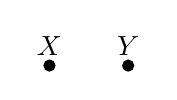
\begin{tikzpicture}
    \filldraw[black] (0,0) circle (2pt) node[anchor=south]{$X$};
    \filldraw[black] (1,0) circle (2pt) node[anchor=south]{$Y$};
  \end{tikzpicture}
\end{center}

A morphism $f$ between, say, $X \otimes Y$ and $A \otimes B \otimes C$ can be drawn as a diagram consisting of some lines and boxes.

\begin{center}
  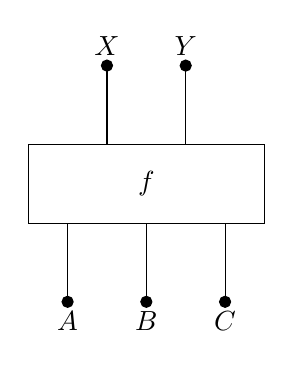
\begin{tikzpicture}
    \filldraw[black] (-0.5,0) circle (2pt) node[anchor=south]{$X$};
    \filldraw[black] (0.5,0) circle (2pt) node[anchor=south]{$Y$};
    \draw (-0.5, 0) -- (-0.5, -1);
    \draw (0.5, 0) -- (0.5, -1);
    \draw (-1.5, -1) -- (-1.5, -2) -- (1.5, -2) -- (1.5, -1) -- cycle;
    \draw (-1, -2) -- (-1, -3);
    \draw (0, -2) -- (0, -3);
    \draw (1, -2) -- (1, -3);
    \draw (0,-1.5) node{$f$};
    \filldraw[black] (-1,-3) circle (2pt) node[anchor=north]{$A$};
    \filldraw[black] (0,-3) circle (2pt) node[anchor=north]{$B$};
    \filldraw[black] (1,-3) circle (2pt) node[anchor=north]{$C$};
  \end{tikzpicture}
\end{center}

We can compose morphisms by concatenating their diagrams.
\begin{center}
  \begin{tikzpicture}
    \filldraw[black] (-0.5,0) circle (2pt) node[anchor=south]{$X$};
    \filldraw[black] (0.5,0) circle (2pt) node[anchor=south]{$Y$};
    \draw (-0.5, 0) -- (-0.5, -1);
    \draw (0.5, 0) -- (0.5, -1);
    \draw (-1.5, -1) -- (-1.5, -2) -- (1.5, -2) -- (1.5, -1) -- cycle;
    \draw (-1, -2) -- (-1, -3);
    \draw (0, -2) -- (0, -3);
    \draw (1, -2) -- (1, -3);
    \draw (0,-1.5) node{$f$};
    \draw (-1.5, -4) -- (-1.5, -3) -- (1.5, -3) -- (1.5, -4) -- cycle;
    \draw (0,-3.5) node{$g$};
    \draw (0, -4) -- (0, -5);
    \filldraw[black] (0, -5) circle (2pt) node[anchor=north]{$Z$};
  \end{tikzpicture}
\end{center}

In a braided monoidal category, we require that for any two objects $X$ and $Y$ we have an isomorphism $\gamma_{XY}\colon X \otimes Y \to Y \otimes X$, which we draw like this.

\begin{center}
  \begin{tikzpicture}
    \braid (braid) s_1;
    \node[at=(braid-1-s), anchor=south]{$X$};
    \node[at=(braid-2-s), anchor=south]{$Y$};
    \node[at=(braid-1-e), anchor=north]{$X$};
    \node[at=(braid-2-e), anchor=north]{$Y$};
  \end{tikzpicture}
\end{center}

Since $\gamma_{AB}$ is an isomorphism, it has an inverse $\gamma_{AB}^{-1}$ (not necessarily equal to $\gamma_{BA}$!) which we draw like this.

\begin{center}
  \begin{tikzpicture}
    \braid (braid) s_{1}^{-1};
    \node[at=(braid-1-s), anchor=south]{$X$};
    \node[at=(braid-2-s), anchor=south]{$Y$};
    \node[at=(braid-1-e), anchor=north]{$X$};
    \node[at=(braid-2-e), anchor=north]{$Y$};
  \end{tikzpicture}
\end{center}

The idea of a braided monoidal category is that we want to take these pictures seriously: we want two expressions involving repeated applications of the $\gamma_{\cdot\cdot}$ and their inverses to be equivalent if and only if the braid diagrams representing them are homotopic. Thus we want, for example,
\begin{equation*}
  \gamma_{XY} \circ \gamma_{YZ} \circ \gamma_{XY} =  \gamma_{YZ} \circ \gamma_{XY} \circ \gamma_{YZ}
\end{equation*}
since
\begin{equation*}
  \begin{aligned}
    \begin{tikzpicture}
      \braid (braid) s_1 s_{2} s_{1};
      \node[at=(braid-1-s), anchor=south]{$X$};
      \node[at=(braid-2-s), anchor=south]{$Y$};
      \node[at=(braid-3-s), anchor=south]{$Z$};
      \node[at=(braid-1-e), anchor=north]{$X$};
      \node[at=(braid-2-e), anchor=north]{$Y$};
      \node[at=(braid-3-e), anchor=north]{$Z$};
    \end{tikzpicture}
  \end{aligned}
  \qquad\text{is homotopic to}\qquad
  \begin{aligned}
    \begin{tikzpicture}
      \braid (braid) s_2 s_{1} s_{2};
      \node[at=(braid-1-s), anchor=south]{$X$};
      \node[at=(braid-2-s), anchor=south]{$Y$};
      \node[at=(braid-3-s), anchor=south]{$Z$};
      \node[at=(braid-1-e), anchor=north]{$X$};
      \node[at=(braid-2-e), anchor=north]{$Y$};
      \node[at=(braid-3-e), anchor=north]{$Z$};
    \end{tikzpicture}
  \end{aligned}
  .
\end{equation*}

A digression into the theory of braid groups would take us too far afield. The punchline is that to guarantee that all such compositions involving the $\gamma$ are identified in the correct way, we must define braided monoidal categories as follows.

\begin{definition}[braided monoidal category]
  \label{def:braidedmonoidalcategory}
  A catgory $\mathsf{C}$ with monoidal structure $(\otimes, 1, \alpha, \lambda, \rho)$ is \defn{braided} if for every two objects $A$ and $B \in \Obj(\mathsf{C})$, there is an isomorphism $\gamma_{A,B}\colon A \otimes B \to B \otimes A$ such that the following \emph{hexagon diagrams} commute.
  \begin{equation*}
    \begin{tikzcd}
      & A \otimes (B \otimes C) \arrow[r, "{\gamma_{A, B \otimes C}}"] & (B \otimes C) \otimes A \arrow[dr, "\alpha_{BCA}"] & \\
      (A \otimes B) \otimes C \arrow[ur, "\alpha_{ABC}"] \arrow[dr, swap, "\gamma_{AB} \otimes 1"] & & & B \otimes (C \otimes A) \\
      & (B \otimes A) \otimes C \arrow[r, swap, "\alpha_{BAC}"] & B \otimes (A \otimes C) \arrow[ur, swap, "1 \otimes \gamma"]
    \end{tikzcd}
  \end{equation*}
  \begin{equation*}
    \begin{tikzcd}
      & (A \otimes B) \otimes C \arrow[r, "{\gamma_{A \otimes B, C}}"] & C \otimes (A \otimes B) \arrow[dr, "\alpha^{-1}_{CAB}"] \\
      A \otimes (B \otimes C) \arrow[ur, "\alpha_{ABC}^{-1}"] \arrow[dr, swap, "1 \otimes \gamma_{BC}"] & & & (C \otimes A) \otimes B \\
      & A \otimes (C \otimes B) \arrow[r, swap, "\alpha^{-1}_{ACB}"] & (A \otimes C) \otimes B \arrow[ur, swap, "\gamma_{AC} \otimes 1"]
    \end{tikzcd}
  \end{equation*}
  The collection of such $\gamma$ form a natural isomorphism betweem the bifunctors
  \begin{equation*}
    (A, B) \mapsto A \otimes B\qquad\text{and}\qquad (A,B) \mapsto B \otimes A,
  \end{equation*}
  and is called a \defn{braiding}.
\end{definition}

\begin{definition}[braided monoidal functor]
  \label{def:braidedmonoidalfunctor}
  A lax monoidal functor $(\mathcal{F}, \Phi, \phi)$ (\hyperref[def:monoidalfunctor]{Definition~\ref*{def:monoidalfunctor}}) is \defn{braided monoidal} if it makes the following diagram commute.
  \begin{equation*}
    \begin{tikzcd}[row sep=huge, column sep=huge]
      \mathcal{F}(x) \otimes \mathcal{F}(y)
      \arrow[r, "{\gamma_{\mathcal{F}(x), \mathcal{F}(y)}}"]
      \arrow[d, swap, "{\Phi_{x,  y}}"]
      & \mathcal{F}(y) \otimes \mathcal{F}(x)
      \arrow[d, "{\Phi_{x, y}}"]
      \\
      \mathcal{F}(x \otimes y)
      \arrow[r, "{\mathcal{F}(\gamma_{x, y})}"]
      & \mathcal{F}(y \otimes x)
    \end{tikzcd}
  \end{equation*}
  \begin{note}
    There are no extra conditions imposed on a monoidal natural transformation to turn it into a braided natural transformation.
  \end{note}
\end{definition}


\subsection{Symmetric monoidal categories}

Until now, we have been calling the bifunctor $\otimes$ in \hyperref[def:monoidalcategory]{Definition~\ref*{def:monoidalcategory}} a tensor product. This has been an abuse of terminology: in general, one defines tensor products not to be those bifunctors which come from any monoidal category, but only those which come from \emph{symmetric} monoidal categories. We will define these shortly.

Conceptually, passing from the definition of a braided monoidal category to that of a symmetric monoidal category is rather simple. One only requires that for any two objects $A$ and $B$, $\gamma_{BA} = \gamma_{AB}^{-1}$, i.e. $\gamma_{BA} \circ \gamma_{AB} = \id_{A \otimes B}$.

We can interpret this nicely in terms of our braid diagrams. We can draw $\gamma_{BA} \circ \gamma_{AB}$ like this.

\begin{center}
  \begin{tikzpicture}
    \braid (braid) s_1 s_1;
    \node[at=(braid-1-s), anchor=south]{$A$};
    \node[at=(braid-2-s), anchor=south]{$B$};
    \node[at=(braid-1-e), anchor=north]{$A$};
    \node[at=(braid-2-e), anchor=north]{$B$};
  \end{tikzpicture}
\end{center}

The requirement that this must be homotopic to the identity transformation
\begin{center}
  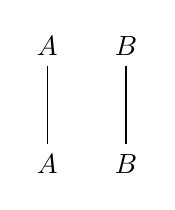
\begin{tikzpicture}
    \draw (0,0) node[anchor=south]{$A$} -- (0,-1) node[anchor=north]{$A$};
    \draw (1,0) node[anchor=south]{$B$} -- (1,-1) node[anchor=north]{$B$};
  \end{tikzpicture}
\end{center}

can be expressed by making the following rule: in a \emph{symmetric} monoidal category, we don't care about the difference between undercrossings and overcrossings:
\begin{equation*}
  \begin{aligned}
    \begin{tikzpicture}
      \braid (braid) s_1;
      \node[at=(braid-1-s), anchor=south]{$A$};
      \node[at=(braid-2-s), anchor=south]{$B$};
      \node[at=(braid-1-e), anchor=north]{$A$};
      \node[at=(braid-2-e), anchor=north]{$B$};
    \end{tikzpicture}
  \end{aligned}
  \qquad = \qquad
  \begin{aligned}
    \begin{tikzpicture}
      \braid (braid) s_1^{-1};
      \node[at=(braid-1-s), anchor=south]{$A$};
      \node[at=(braid-2-s), anchor=south]{$B$};
      \node[at=(braid-1-e), anchor=north]{$A$};
      \node[at=(braid-2-e), anchor=north]{$B$};
    \end{tikzpicture}
  \end{aligned}
  .
\end{equation*}

Then we can exchange the diagram representing $\gamma_{BA} \circ \gamma_{AB}$ for

\begin{center}
  \begin{tikzpicture}
    \braid (braid) s_1 s_1^{-1};
    \node[at=(braid-1-s), anchor=south]{$A$};
    \node[at=(braid-2-s), anchor=south]{$B$};
    \node[at=(braid-1-e), anchor=north]{$A$};
    \node[at=(braid-2-e), anchor=north]{$B$};
  \end{tikzpicture}
\end{center}
which is clearly homotopic to the identity transformation on $A \otimes B$.

\begin{definition}[symmetric monoidal category]
  \label{def:symmetricmonoidalcategory}
  Let $\mathsf{C}$ be a braided monoidal category with braiding $\gamma$. We say that $\mathsf{C}$ is a \defn{symmetric monoidal category} if for all $A$, $B \in \Obj(\mathsf{C})$, $\gamma_{BA} \circ \gamma_{AB} = \id_{A \otimes B}$. A braiding $\gamma$ which satisfies such a condition is called \defn{symmetric}.
\end{definition}

\begin{note}
  There are no extra conditions imposed on a monoidal natural transformation to turn it into a symmetric natural transformation.
\end{note}


\section{Internal hom functors}\label{sec:internalhomfunctors}

We can now generalize the notion of an exponential object (\hyperref[def:exponential]{Definiton~\ref*{def:exponential}}) to any monoidal category.


\subsection{The internal hom functor}

Recall the definition of the hom functor on a locally small category $\mathsf{C}$ (\hyperref[def:homfunctor]{Definition~\ref*{def:homfunctor}}): it is the functor which maps two objects to the set of morphisms between them, so it is a functor
\begin{equation*}
  \mathsf{C}^{\mathrm{op}} \times \mathsf{C} \rightsquigarrow \mathsf{Set}.
\end{equation*}

If we take $\mathsf{C} = \mathsf{Set}$, then our hom functor never really leaves $\mathsf{Set}$; it is \emph{internal} to $\mathsf{Set}$. This is our first example of an \emph{internal hom functor}. In fact, it is the prototypical internal hom functor, and we can learn a lot by studying its properties.

Let $X$ and $Y$ be sets. Denote the set of all functions $X \to Y$ by $[X,Y]$.

Let $S$ be any other set, and consider a function $f\colon S \to [X, Y]$. For each element $s \in S$, $f$ picks out a function $h_{s}\colon X \to Y$. But this is just a curried version of a function $S \times X \to Y$! So as we saw in \hyperref[section:homfunctor]{Section~\ref*{section:homfunctor}}, we have a bijection between the sets $[S, [X, Y]]$ and $[S \times X, Y]$. In fact, this is even a \emph{natural} bijection, i.e.\ a natural transformation between the functors
\begin{equation*}
  [-,[-,-]]\qquad \text{and}\quad [- \times -, -]\colon \mathsf{Set}^{\mathrm{op}} \times \mathsf{Set}^{\mathrm{op}} \times \mathsf{Set} \rightsquigarrow \mathsf{Set}.
\end{equation*}

Let's check this. First, we need to figure out how our functors act on functions. Suppose we have sets and functions like so.
\begin{equation*}
  \begin{tikzcd}[row sep=tiny]
    A''
    & B''
    \arrow[l, swap, "f''"]
    \\
    A'
    & B'
    \arrow[l, swap, "f'"]
    \\
    A
    \arrow[r, "f"]
    & B
  \end{tikzcd}
\end{equation*}
Our functor maps
\begin{equation*}
  (A'', A', A) \mapsto [A'', [A', A]] = \Hom_{\mathsf{Set}}(A'', \Hom_{\mathsf{Set}}(A', A)),
\end{equation*}
so it should map $(f'', f', f)$ to a function
\begin{equation*}
  [f'', [f', f]]\colon [A'', [A', A]] \to [B'', [B', B]].
\end{equation*}
The way to do that is by sending $m \in [A'', [A', A]]$ to
\begin{equation*}
  [f', f] \circ m \circ f''.
\end{equation*}
You can check that this works as advertised.

The other one's not so tough. Our functor maps an object $(A'', A', A)$ to $[A'' \times A', A]$. We need to map $(f'', f', f)$ to a function
\begin{equation*}
  [f'' \times f' , f]\colon [A'' \times A', A] \to [B'' \times B', B].
\end{equation*}
We do that by sending $m \in [A'' \times A', A]$ to
\begin{equation*}
  f \circ m \circ (f'', f') \in [B'' \times B', B].
\end{equation*}

Checking that $[-,[-,-]]$ and $[-\times-, -]$ really \emph{are} functorial would be a bit much; each is just the composition of hom functor and the Cartesian product. We will however check that there is a natural isomorphism between them, which amounts to checking that the following diagram commutes.
\begin{equation*}
  \begin{tikzcd}[column sep=0.9]
    {[A'' \times A', A]}
    \arrow[rrr, "{[f'' \times f', f]}"]
    \arrow[ddd, swap, "{\Phi_{[A'' \times A', A]}}"]
    & & & {[B'' \times B', B]}
    \arrow[ddd, "{\Phi_{[B'' \times B', B]}}"]
    \\
    & m
    \arrow[d, mapsto]
    \arrow[r, mapsto]
    & f \circ m \circ (f', f'')
    \arrow[d, mapsto]
    \\
    & \Phi(m)
    \arrow[r, mapsto]
    & {[f', f] \circ \Phi(m) \circ f'' \stackrel{!}{=} \Phi(f \circ m \circ (f', f''))}
    \\
    {[A'', [A', A]]}
    \arrow[rrr, swap, "{[f'', [f', f]]}"]
    & & & {[B'', [B', B]]}
  \end{tikzcd}
\end{equation*}
In other words, we have to show that
\begin{equation*}
  \Phi_{[A'' \times A', A]}(f \circ m \circ (f', f'')) = [f', f] \circ \Phi_{[B'' \times B', B]}(m) \circ f''.
\end{equation*}

So what is each of these? Well, $f \circ m \circ (f', f'')$ is a map $B'' \times B' \to B$, which maps (say) $(b'', b') \mapsto b$.

The natural transformation $\Phi$ tells us to curry this, i.e.\ turn it into a map $B'' \to [B', B]$. Not just any map, though: a map which when evaluated on $b''$ turns into a map which, when evaluated on $b'$, yields $b$.

We know that $f \circ m \circ (f', f'')\colon (b'', b') \mapsto b$, i.e.
\begin{equation*}
  f(m(f''(b''), f'(b'))) = b.
\end{equation*}
If we can show that this is \emph{also} what $[f', f] \circ \Phi_{[B'' \times B', B]}(m) \circ f''$ is equal to when evaluated on $b''$ and then $b'$, we are done, since two functions are equal if they take the same value for all inputs.

Well, let's go through what this definition means. First, we take $b''$ and feed it to $f''$. Next, we let $\Phi_{[B'' \times B', B]}(m)$ act on the result, i.e.\ we fill the first argument of $m$ with $f''(b'')$. What we get is the following:
\begin{equation*}
  m(f''(b''), -).
\end{equation*}
Then we are to precompose this with $f'$ and stick the result into $f$:
\begin{equation*}
  f(m(f''(b''), f'(-))).
\end{equation*}
Finally, we are to evaluate this on $b'$ to get
\begin{equation*}
  f(m(f''(b''), f'(b'))).
\end{equation*}

Indeed, this is equal to $b$, so the diagram commutes.

In other words, $\Phi$ is a natural bijection between the hom-sets $[-,[-,-]]$ and $[- \times -, -]$.

We picked this example because the collection $[A, B]$ of all functions between two sets $A$ and $B$ is itself a set. Therefore it makes sense to think of the hom-sets $\Hom_{\mathsf{C}}(A, B)$ as living within the same category as $A$ and $B$. We saw in \hyperref[sec:cartesianclosedcategories]{Section~\ref*{sec:cartesianclosedcategories}} that in a category with products, we could sometimes view hom-sets as exponential objects. However, we now have the technology to be even more general.

\begin{definition}[internal hom functor]
  \label{def:internalhomfunctor}
  Let $(\mathsf{C}, \otimes)$ be a monoidal category. An \defn{internal hom functor} is a functor
  \begin{equation*}
    {[-, -]}_{\mathsf{C}}\colon \mathsf{C}^{\mathrm{op}} \times \mathsf{C} \rightsquigarrow \mathsf{C}
  \end{equation*}
  such that for every $X \in \Obj(\mathsf{C})$ we have a pair of adjoint functors
  \begin{equation*}
    (-) \otimes X \dashv {[X, -]}_{\mathsf{C}}.
  \end{equation*}

  The objects ${[A, B]}_{\mathsf{C}}$ are called \defn{internal hom objects}.
\end{definition}

\begin{note}
  The reason for the long introduction to this section was that the pair of adjoint functors in \hyperref[def:internalhomfunctor]{Definition~\ref*{def:internalhomfunctor}} really matches the one in $\mathsf{Set}$. Recall, in $\mathsf{Set}$ there was a natural transformation
  \begin{equation*}
    \Hom_{\mathsf{Set}}(S \times X, Y) \simeq \Hom_{\mathsf{Set}}(S, [X, Y]).
  \end{equation*}

  This means that for any set $X$, there is a pair of adjoint functors
  \begin{equation*}
    (-) \times X \dashv [X, -],
  \end{equation*}
  which is in agreement with the statement of \hyperref[def:internalhomfunctor]{Definition~\ref*{def:internalhomfunctor}}.
\end{note}

\begin{notation}
  The convention at the nLab is to denote the internal hom by square braces $[A,B]$, and this is for the most part what we will do. Unfortunately, we have already used this notation for the \emph{regular} hom functor. To remedy this, we will add a subscript if the category to which the hom functor belongs is not clear: ${[-,-]}_{\mathsf{C}}$ for a hom functor internal to $\mathsf{C}$, ${[-,-]}_{\mathsf{Set}}$ for the standard hom functor (or the hom functor internal to $\mathsf{Set}$, which amounts to the same).

  There is no universally accepted notation for the internal hom functor. One often sees it denoted by a lower-case $\hom$: $\hom_{\mathsf{C}}(A, B)$. Many sources (for example DMOS~\cite{DMOS}) distinguish the internal hom with an underline: $\underline{\Hom}_{\mathsf{C}}(A, B)$. Deligne typesets it with a script H\@: $\mathscr{H}om_{\mathsf{C}}(A, B)$.
\end{notation}

\begin{definition}[closed monoidal category]
  \label{def:closedmonoidalcategory}
  A monoidal category equipped with an internal hom functor is called a \defn{closed monoidal category}.
\end{definition}

\begin{note}
  Here is another (clearly equivalent) definition of ${[X, Y]}_{\mathsf{C}}$: it is the object representing (\hyperref[def:representablefunctor]{Definition~\ref*{def:representablefunctor}}) the functor
  \begin{equation*}
    T \mapsto \Hom_\mathsf{C}(T \otimes X, Y).
  \end{equation*}
\end{note}

\begin{example}
  In many locally small categories whose objects can be thought of as ``sets with extra structure,'' it is possible to pile structure on top of the hom sets until they themselves can be viewed as bona fide objects in their categories. It often (\emph{but not always!}) happens that these beefed-up hom sets coincide (up to isomorphism) with the internal hom objects.

  Take for example $\mathsf{Vect}_{k}$. For any vector spaces $V$ and $W$, we can turn $\Hom_{\mathsf{Vect}_{k}}(V, W)$ into a vector space by defining addition and scalar multiplication pointwise; we can then view $\Hom_{\mathsf{Vect}_{k}}(V, W)$ as belonging to $\Obj(\mathsf{Vect}_{k})$. It turns out that this is precisely (up to isomorphism) the internal hom object ${[V, W]}_{\mathsf{Vect}_{k}}$.

  To see this, we need to show that there is a natural bijection
  \begin{equation*}
    \Hom_{\mathsf{Vect}_{k}}(A, \Hom_{\mathsf{Vect}_{k}}(B, C)) \simeq \Hom_{\mathsf{Vect}_{k}}(A \otimes B, C).
  \end{equation*}

  Suppose we are given a linear map $f\colon A \to \Hom_{\mathsf{Vect}_{k}}(B, C)$. If we act with this on an element of $A$, we get a linear map $B \to C$. If we evaluate this on an element of $B$, we get an element of $C$. Thus, we can view $f$ as a bilinear map $A \times B \to C$, hence as a linear map $A \otimes B \to C$.

  Now suppose we are given a linear map $g\colon A \otimes B \to C$. By pre-composing this with the tensor product we can view this as a bilinear map $A \times B \to C$, and by currying this we get a linear map $A \to \Hom_{\mathsf{Vect}_{k}}(B, C)$.
\end{example}

For the remainder of this chapter, let $(\mathsf{C}, \otimes, 1)$ be a closed monoidal category with internal hom functor ${[-,-]}_{\mathsf{C}}$.

In a closed monoidal category, the adjunction between the internal hom and the tensor product even holds internally.
\begin{lemma}
  For any $X$, $Y$, $Z \in \Obj(\mathsf{C})$ there is a natural isomorphism
  \begin{equation*}
    {[X \otimes Y, Z]}_{\mathsf{C}} \stackrel{\sim}{\to} {[X, {[Y, Z]}_{\mathsf{C}}]}_{\mathsf{C}}.
  \end{equation*}
\end{lemma}
\begin{proof}
  Let $A \in \Obj(\mathsf{C})$. We have the following string of natural isomorphisms.
  \begin{align*}
    \Hom_{\mathsf{C}}(A, {[X \otimes Y, Z]}_{\mathsf{C}}) &\simeq \Hom_{\mathsf{C}}(A \otimes (X \otimes Y), Z) \\
    &\simeq \Hom_{\mathsf{C}}((A \otimes X) \otimes Y, Z) \\
    &\simeq \Hom_{\mathsf{C}}(A \otimes X, {[Y, Z]}_{\mathsf{C}}) \\
    &\simeq \Hom_{\mathsf{C}}(A, {[X, {[Y, Z]}_{\mathsf{C}}]}_{\mathsf{C}}).
  \end{align*}

  Since this is true for each $A$ we have, by \hyperref[cor:yonedaembeddingrespectsisomorphisms]{Corollary~\ref*{cor:yonedaembeddingrespectsisomorphisms}},
  \begin{equation*}
    {[X \otimes Y, Z]}_{\mathsf{C}} \stackrel{\sim}{\to} {[X, {[Y, Z]}_{\mathsf{C}}]}_{\mathsf{C}}.
  \end{equation*}
\end{proof}

\begin{lemma}
  \label{lemma:cantensorbothsidesofinternalhom}
  Let $(\mathsf{C}, \otimes, 1)$ be a closed symmetric monoidal category. For any $A$, $B$, $R \in \Obj(\mathsf{C})$, there is a natural transformation
  \begin{equation*}
    {[A, B]}_{\mathsf{C}} \to {[R \otimes A, R \otimes B]}_{\mathsf{C}},
  \end{equation*}
  natural in $A$ and $B$.
\end{lemma}
\begin{proof}
  The assignment $R \otimes (-)$ is a functor, and induces a transformation of the regular hom functor
  \begin{equation*}
    \Hom_{\mathsf{C}}(A, B) \mapsto \Hom_{\mathsf{C}}(R \otimes A, R \otimes B)
  \end{equation*}
  which is natural in $A$ and $B$. We would like to show that the internal hom functor also has this property.

  The following string of natural transformations guarantees it by the Yoneda lemma.
  \begin{align*}
    \Hom_{\mathsf{C}}(X, {[A, B]}_{\mathsf{C}}) &\simeq \Hom_{\mathsf{C}}(X \otimes A, \otimes B) \\
    &\simeq \Hom_{\mathsf{C}}(R \otimes X \otimes A, R \otimes B) \\
    &\simeq \Hom_{\mathsf{C}}(X \otimes (R \otimes A), R \otimes B) \\
    & \simeq \Hom_{\mathsf{C}}(X, {[R \otimes A, R \otimes B]}_{\mathsf{C}}).
  \end{align*}
\end{proof}


\subsection{The evaluation map}

The internal hom functor gives us a way to talk about evaluating morphisms $f\colon X \to Y$ without mentioning elements of $X$.
\begin{definition}[evaluation map]
  \label{def:evaluationmap}
  Let $X \in \Obj(\mathsf{C})$. We have seen that the adjunction
  \begin{equation*}
    (-) \otimes X \dashv {[X, -]}_{\mathsf{C}}
  \end{equation*}
  gives us, for any $A$, $X$, $Y \in \Obj(\mathsf{C})$, a natural bijection
  \begin{equation*}
    \Hom_{\mathsf{C}}(A \otimes X, Y) \overset{\sim}{\to} \Hom_{\mathsf{C}}(A, {[X, Y]}_{\mathsf{C}}).
  \end{equation*}
  In particular, with $A = {[X, Y]}_{\mathsf{C}}$, we have a bijection
  \begin{equation*}
    \Hom_{\mathsf{C}}({[X, Y]}_{\mathsf{C}} \otimes X, Y) \overset{\sim}{\to} \Hom_{\mathsf{C}}({[X, Y]}_{\mathsf{C}}, {[X, Y]}_{\mathsf{C}}).
  \end{equation*}

  The adjunct (\hyperref[def:adjunct]{Definition~\ref*{def:adjunct}}) of $\id_{{[X, Y]}_{\mathsf{C}}} \in \Hom_{\mathsf{C}}({[X, Y]}_{\mathsf{C}}, {[X, Y]}_{\mathsf{C}})$ is an object in $\Hom_{\mathsf{C}}\left( {[X, Y]}_{\mathsf{C}} \otimes X, Y \right)$, denoted
  \begin{equation*}
    \ev_{X, Y}\colon {[X, Y]}_{\mathsf{C}} \otimes X \to Y,
  \end{equation*}
  and called the \defn{evaluation map}.
\end{definition}

\begin{example}
  \label{eg:evaluationmapinset}
  As we saw in \hyperref[eg:setisamonoidalcategory]{Example~\ref*{eg:setisamonoidalcategory}}, the category $\mathsf{Set}$ is a monoidal category with a bifunctor given by the cartesian product. The internal hom is simply the regular hom functor
  \begin{equation*}
    \Hom_{\mathsf{Set}}(-,-) = [-,-].
  \end{equation*}
  Let us explore the evaluation map on $\mathsf{Set}$. It is the adjunct of the identity map $\id_{[X, Y]}$ under the adjunction
  \begin{equation*}
    [[X, Y] \times X, Y] \dashv [[X, Y], [X, Y]].
  \end{equation*}
  Thus, it is a function
  \begin{equation*}
    \ev_{X, Y}\colon [X, Y] \times X \to Y;\qquad (f, x) \mapsto \ev_{X, Y}(f, x).
  \end{equation*}
  So far, we don't know what $\ev_{X, Y}$ sends $(f, x)$ to; we just know that we'd \emph{like it} if it sent it to $f(x)$.

  The above adjunction is given by currying: we start on the LHS with a map $\ev_{X, Y}$ with two arguments, and we turn it into a map which fills in only the first argument. Thus the map on the RHS adjunct to $\ev_{X, Y}$ is given by
  \begin{equation*}
    f \mapsto \ev_{X, Y}(f, -).
  \end{equation*}
  If we want the map $f \mapsto \ev_{X, Y}(f, -)$ to be the identity map, $f$ and $\ev_{X, Y}(f, -)$ must agree on all elements $x$, i.e.
  \begin{equation*}
    f(x) = \ev_{X, Y}(f, x)\qquad\text{for all }x \in X.
  \end{equation*}
  Thus, the evaluation map is the map which sends $(f, x) \mapsto f(x)$.
\end{example}


\subsection{The composition morphism}

The evaluation map allows us to define composition of morphisms without talking about internal hom objects as if they have elements.
\begin{definition}[composition morphism]
  \label{def:compositionmorphism}
  For $X$, $Y$, $Z \in \Obj(\mathsf{C})$, the \defn{composition morphism}
  \begin{equation*}
    \circ_{X, Y, Z}\colon {[Y, Z]}_{\mathsf{C}} \otimes {[X, Y]}_{\mathsf{C}} \to {[X, Z]}_{\mathsf{C}}
  \end{equation*}
  is the $(-) \otimes X \vdash {[X, -]}_{\mathsf{C}}$-adjunct of the composition
  \begin{equation*}
    \begin{tikzcd}[column sep=huge]
      {[Y, Z]}_{\mathsf{C}} \otimes {[X, Y]}_{\mathsf{C}} \otimes X
      \arrow[r, "{\left(\id_{{[Y, Z]}_{\mathsf{C}}}, \ev_{X, Y}\right)}"]
      & {{[Y, Z]}_{\mathsf{C}}} \otimes Y
      \arrow[r, "{\ev_{Y, Z}}"]
      & Z
    \end{tikzcd}.
  \end{equation*}
\end{definition}

\begin{example}
  In $\mathsf{Set}$, the composition morphism $\circ_{X, Y, Z}$ lives up to its name. Let $f\colon X \to Y$, $g\colon Y \to Z$, and $x \in X$. The above composition goes as follows.
  \begin{enumerate}
    \item The map $\left( \id_{[Y, Z]}, \ev_{X, Y} \right)$ turns the triple $(g, f, x)$ into the pair $(g, f(x))$.

    \item The map $\ev_{Y, Z}$ turns $(g, f(x))$ into $g(f(x)) = (g \circ f)(x)$.
  \end{enumerate}

  The evaluation morphism $\circ_{X, Y, Z}$ is the currying of this, i.e.\ it sends
  \begin{equation*}
    (f, g) \mapsto (f \circ g)(-).
  \end{equation*}
\end{example}


\subsection{Dual objects}

Recall that for any $k$-vector space $V$, there is a dual vector space
\begin{equation*}
  V^{*} = \left\{ L\colon V \to k \right\}.
\end{equation*}
This definition generalizes to any closed monoidal category.

\begin{definition}[dual object]
  \label{def:dualobject}
  Let $X \in \Obj(\mathsf{C})$. The \defn{dual object} to $X$, denoted $X^{*}$, is defined to be the object
  \begin{equation*}
    {[X, 1]}_{\mathsf{C}}.
  \end{equation*}

  That is to say, $X^{*}$ is the internal hom object modelling the hom set of morphisms from $X$ to the identity object $1$.
\end{definition}

\begin{notation}
  The evaluation morphism (\hyperref[def:evaluationmap]{Definition~\ref*{def:evaluationmap}}) has a component
  \begin{equation*}
    \ev_{X^{*}, X}\colon X^{*} \otimes X \to 1.
  \end{equation*}

  To clean things up a bit, we will write $\ev_{X}$ instead of $\ev_{X^{*}, X}$.
\end{notation}

\begin{notation}
  In many sources, e.g. DMOS (\cite{DMOS}), the dual object to $X$ is denoted $X^{\vee}$ instead of $X^{*}$.
\end{notation}

\begin{lemma}
  There is a natural isomorphism between the functors
  \begin{equation*}
    \Hom_{\mathsf{C}}(-, X^{*})\qquad\text{and}\qquad \Hom_{\mathsf{C}}((-) \otimes X, 1).
  \end{equation*}
\end{lemma}
\begin{proof}
  For any $X$, $T \in \Obj(\mathsf{C})$, the definition of the internal hom ${[-,-]}_{\mathsf{C}}$ gives us a natural isomorphism
  \begin{equation*}
    \Hom_{\mathsf{C}}(T \otimes X, 1) \simeq \Hom_{\mathsf{C}}(T, {[X, 1]}_{\mathsf{C}}) = \Hom_{\mathsf{C}}(T, X^{*}).
  \end{equation*}
\end{proof}

\begin{theorem}
  The map $X \mapsto X^{*}$ can be extended to a contravariant functor.
\end{theorem}
\begin{proof}
  We need to figure out how our functor should act on morphisms. We define this by analogy with the familiar setting of vector spaces. Recall that for a linear map $L\colon V \to W$, the dual map $L^{t}\colon W^{*} \to V^{*}$ is defined by
  \begin{equation*}
    (L^{t}(w))(v) = w(L(v)).
  \end{equation*}

  By analogy, for $f \in \Hom_{\mathsf{C}}(X, Y)$, we should define the dual morphism $f^{t} \in \Hom_{\mathsf{C}}(B^{*}, A^{*})$ by demanding that the following diagram commutes.
  \begin{equation*}
    \begin{tikzcd}[row sep=huge, column sep=huge]
      h^{*} \otimes X
      \arrow[r, "f^{t} \otimes \id_{X}"]
      \arrow[d, swap, "\id_{Y} \otimes f"]
      & X^{*} \otimes X
      \arrow[d, "\ev_{X}"]
      \\
      h^{*} \otimes Y
      \arrow[r, "\ev_{Y}"]
      & 1
    \end{tikzcd}
  \end{equation*}

  To check that this is functorial, we must check that it respects compositions, i.e.\ that the following diagram commutes.
  \begin{equation*}
    \begin{tikzcd}[row sep=huge, column sep=huge]
      Z^{*} \otimes X
      \arrow[r, "(f^{t} \circ g^{t}) \otimes \id_{X}"]
      \arrow[d, swap, "\id_{Z} \otimes (g \circ f)"]
      & X^{*} \otimes X
      \arrow[d, "\ev_{X}"]
      \\
      Z^{*} \otimes Z
      \arrow[r, "\ev_{Z}"]
      & 1
    \end{tikzcd}
  \end{equation*}

  Let's add in some more objects and morphisms.
  \begin{equation*}
    \begin{tikzcd}[row sep=huge, column sep=huge]
      Z^{*} \otimes X
      \arrow[r, "g^{t} \otimes \id_{X}"]
      \arrow[d, swap, "\id_{Z^{*}} \otimes f"]
      & h^{*} \otimes X
      \arrow[r, "f^{t} \otimes \id_{X}"]
      \arrow[d, swap, "\id_{h^{*}} \otimes f"]
      & X^{*} \otimes X
      \arrow[dd, "\ev_{X}"]
      \\
      Z^{*} \otimes Y
      \arrow[r, "g^{t} \otimes \id_{Y}"]
      \arrow[d, swap, "\id_{Z^{*}} \otimes g"]
      & h^{*} \otimes Y
      \arrow[dr, "\ev_{Y}"]
      \\
      Z^{*} \otimes Z
      \arrow[rr, swap, "\ev_{Z}"]
      & & 1
    \end{tikzcd}
  \end{equation*}

  We want to show that the outer square commutes. But it clearly does: that the top left square commutes is trivial, and the right and bottom `squares' are the commutativity conditions defining $f^{t}$ and $g^{t}$.
\end{proof}

\begin{note}
  It's not clear to me why $f^{t}$ as defined above exists and is unique.
\end{note}

The above is one, but not the only, way to define dual objects. We can be more general.
\begin{definition}[right duality]
  \label{def:rightduality}
  Let $\mathsf{C}$ be a category with monoidal structure $(\otimes, 1, \alpha, \lambda, \rho)$. \defn{Right duality} of two objects $A$ and $A^{*} \in \Obj(\mathsf{C})$ consists of
  \begin{enumerate}
    \item A morphism of the form
      \begin{equation*}
        \ev_{A}\colon A^{*} \otimes A \to 1,
      \end{equation*}
      called the \emph{evaluation map} (or \emph{counit} if you're into Hopf algebras)

    \item A morphism of the form
      \begin{equation*}
        i_{A}\colon 1 \to A \otimes A^{*},
      \end{equation*}
      called the \emph{coevaluation} map (or \emph{unit})
  \end{enumerate}
  such that the compositions
  \begin{equation*}
    \begin{tikzcd}[column sep=huge]
      X
      \arrow[r, "i_{A} \otimes \id_{X}"]
      & (X \otimes X^{*}) \otimes X
      \arrow[r, "{\alpha_{X, X^{*}, X}}"]
      & X \otimes (X^{*} \otimes X)
      \arrow[r, "{\id_{X} \otimes \ev_{X}}"]
      & X
      \\
      X^{*}
      \arrow[r, "{\id_{X^{*}} \otimes \ev_{X}}"]
      & X^{*} \otimes (X \otimes X^{*})
      \arrow[r, "{\alpha^{-1}_{X^{*}, X, X^{*}}}"]
      & (X^{*} \otimes X) \otimes X^{*}
      \arrow[r, "{\ev_{X}\otimes \id_{X^{*}}}"]
      & X^{*}
    \end{tikzcd}
  \end{equation*}
  are the identity morphism.
\end{definition}

\begin{definition}[rigid monoidal category]
  \label{def:rigidmonoidalcategory}
  A monoidal category $(\mathsf{C}, \otimes, 1)$ is \defn{rigid} if every object has a left and right dual.
\end{definition}

\begin{theorem}
  Every rigid monoidal category is a closed monoidal category (i.e.\ has an internal hom functor, see \hyperref[def:closedmonoidalcategory]{Definition~\ref*{def:closedmonoidalcategory}}) with internal hom object
  \begin{equation*}
    {[A, B]}_{\mathsf{C}} \simeq B \otimes A^{*}.
  \end{equation*}
\end{theorem}
\begin{proof}
  We can prove the existence of this isomorphism by showing, thanks to \hyperref[cor:yonedaembeddingrespectsisomorphisms]{Corollary~\ref*{cor:yonedaembeddingrespectsisomorphisms}}, that for any $X \in \Obj(\mathsf{C})$ there is an isomorphsm
  \begin{equation*}
    \Hom_{\mathsf{C}}(X, {[A, B]}_{\mathsf{C}}) \simeq \Hom_{\mathsf{C}}(X, B \otimes A^{*}).
  \end{equation*}

  The defining adjunction of the internal hom gives us
  \begin{equation*}
    \Hom_{\mathsf{C}}(X, {[A, B]}_{\mathsf{C}}) \simeq \Hom_{\mathsf{C}}(X \otimes A, B).
  \end{equation*}

  Now we can map any $f \in \Hom_{\mathsf{C}}(X \otimes A, B)$ to
  \begin{equation*}
    (f \otimes \id_{A}) \circ (\id_{X} \otimes i_{A}) \in \Hom_{\mathsf{C}}(X, B \otimes A^{*}).
  \end{equation*}

  We will be done if we can show that the assignment
  \begin{equation*}
    f \mapsto (f \otimes \id_{A}) \circ (\id_{X} \otimes i_{A})
  \end{equation*}
  is an isomorphism. We'll do this by exhibiting an inverse:
  \begin{equation*}
    \Hom_{\mathsf{C}}(X, B \otimes A^{*}) \ni g \mapsto (\id_{W} \otimes \ev_{V}) \circ (g \otimes \id_{V}) \in \Hom_{\mathsf{C}}(X \otimes A, B).
  \end{equation*}

  Of course, first we should show that $(f \otimes \id_{A}) \circ (\id_{X} \otimes i_{A})$ really does map $X \to B \otimes A^{*}$. But it does; it does this by first acting on $X$ with $i_{A}$:
  \begin{equation*}
    X \to X \otimes A \otimes A^{*}
  \end{equation*}
  and then acting on the $X \otimes A$ with $f$ and letting the $A^{*}$ hang around:
  \begin{equation*}
    X \otimes A \otimes A^{*} \to B \otimes A^{*}.
  \end{equation*}

  To show that
  \begin{equation*}
    g \mapsto (\id_{B} \otimes \ev_{A}) \circ (g \otimes \id_{A})
  \end{equation*}
  really is an inverse, we can shove the assignment
  \begin{equation*}
    f \mapsto (f \otimes \id_{A}) \circ (\id_{X} \otimes i_{A})
  \end{equation*}
  into it and show that we get $f$ right back out. That is to say, we need to show that
  \begin{equation*}
    (\id_{B} \otimes \ev_{A}) \circ (\left[ (f \otimes \id_{A}) \circ (\id_{X} \otimes i_{A}) \right] \otimes \id_{A}) = f.
  \end{equation*}
  This is easy to see but hard to type. Write it out. You'll need to use first of the two composition identities.

  To show that the other composition yields $g$, you have to use the other.
\end{proof}


\end{document}
